\documentclass[]{report}
\usepackage[utf8]{inputenc}
\usepackage[spanish]{babel}
\usepackage[nodayofweek,level]{datetime}
\usepackage[left=0.5in, right=0.5in, top=0.7in, bottom=0.7in]{geometry}
\usepackage{graphicx}
\usepackage{amsmath}
\usepackage{changepage}

% Title Page
\title{\Huge\bfseries Proyecto 1: Fase 1}
\author{\Large Universidad Simón Bolívar\\Laboratorio de Bases de Datos CI3391\\ \\Augusto Hidalgo 13-10665\\José Acevedo 13-10006}



\begin{document}%\ttfamily
	\maketitle
	
	\chapter*{Introducción}
	\begin{adjustwidth}{16pt}{16pt}\large
		
		\hspace{1.5em}El siguiente informe describe el proyecto consistente en la elaboración de un sistema de gestión de los procesos de Gerencia de Planta de la empresa BGV C.A. Para ello se modelaron los datos suministrados mediante un diagrama Entidad-Relación Extendido (ER-E). A través de este diagrama se representaron las entidades relevantes
		del sistema de información de BGV C.A., así como sus interrelaciones y propiedades. \\
		
		Se redactó un diccionario de datos para describir los tipos de entidades presentes en el diagrama y sus atributos. De igual manera se describieron las relaciones participantes, especializaciones, generalizaciones y categorizaciones presentes en el modelo. Adicionalmente, se agregaron restricciones explícitas en lenguaje natural y lógico de primer orden para completar las especificaciones de los datos que no pueden ser representadas a través del diagrama ER-E.\\
		
		La modelación conceptual de los datos de BGV C.A. presenta la primera etapa del proyecto de implementación de la base de datos. Posteriormente se realizará la traducción al modelo relacional e implementación de la base de datos para uso de BGV C.A. en la fabricación de bombas de agua.
		
	
\end{adjustwidth}
	
	\chapter*{Diagrama ER-E}
	\begin{center}
		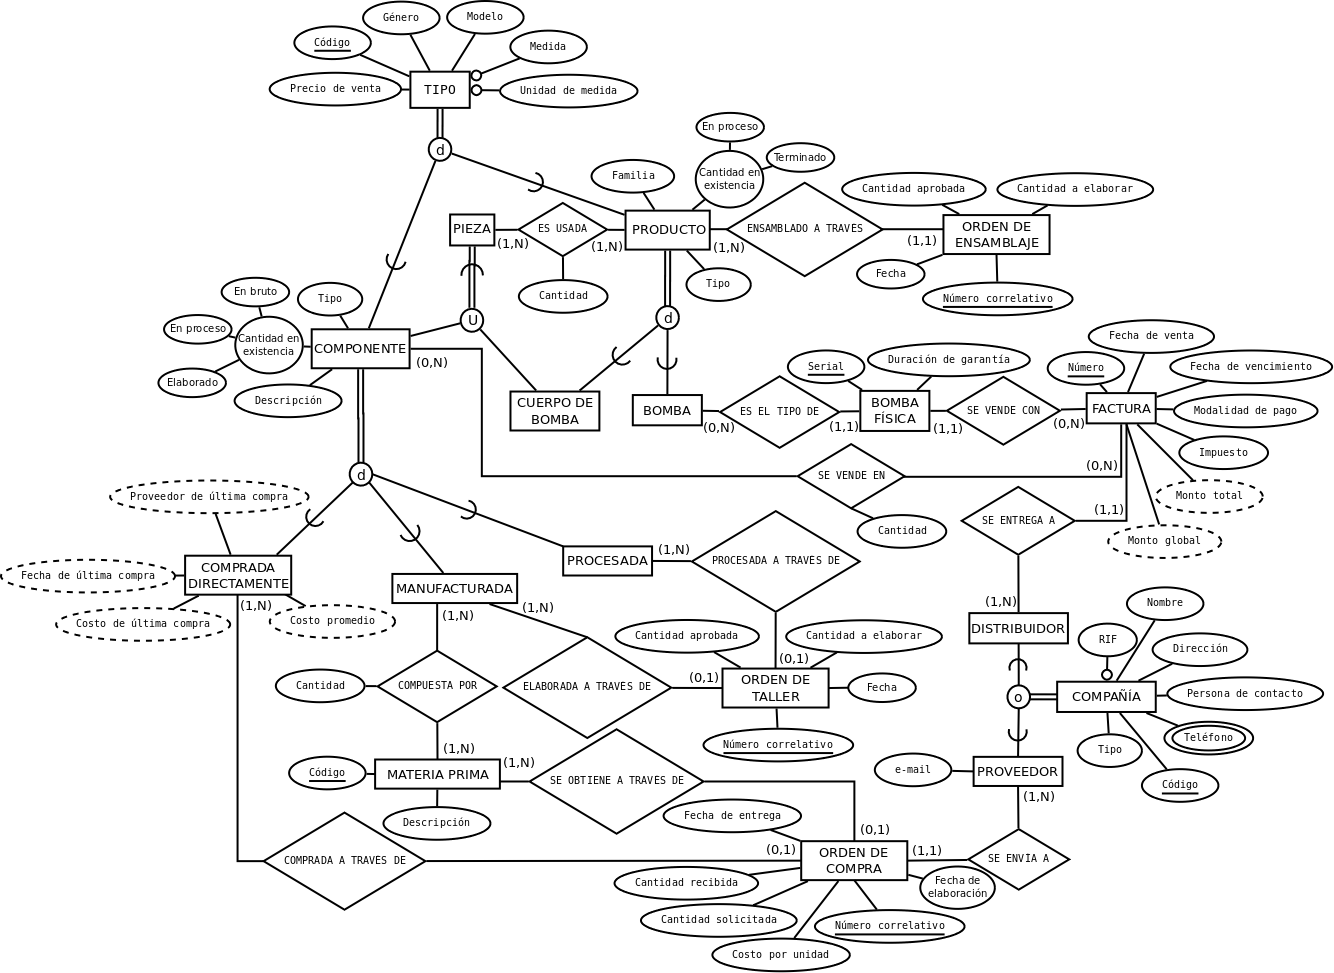
\includegraphics[width=\textwidth,height=\textheight,keepaspectratio]{DiagramFINAL}
	\end{center}
	
	\chapter*{Diccionario de Datos}
	 \section*{\centering Entidades y sus atributos}
	
	\begin{center}
		\begin{tabular}{| p{2.5cm} | p{4.5cm} | p{2cm} | p{5cm} | p{3cm}|}
					\hline
			Entidad & Semántica & Atributos & Semántica de los atributos & Dominio \\ \hline
			
			% TIPO
			TIPO & Engloba cada tipo de producto o componente. & 
			
			Código & Código que identifica cada tipo de componente o producto. & Número de 10 dígitos\\ \cline{3-5}
			&& Modelo & Nombre y descripción del modelo. & String\\ \cline{3-5}
			&& Género & Especifica si es un producto o una componente. & \{'Producto', 'Componente'\} \\ \cline{3-5}
			&& Precio de venta & Precio en Bolívares en el que se vende el producto.& Monto en Bolívares\\ \cline{3-5}
			&& Unidad de medida & Tipo de unidad en la que es medido es producto.&Unidad de longitud, area o volumen\\ \cline{3-5}
			&& Medida & Magnitud en la unidad señalada.& Magnitud positiva\\ \cline{3-5}
			\hline
			
			
			
			COMPONENTE & Tipo de componentes usadas en la producción de bombas. &
			Tipo & Forma de obtención de dicha componente.& \{'Comprada directamente', 'Manufacturada', 'Procesada'\}\\ \cline{3-5}
			&& Descripción & Descripción de la componente.& String\\ \cline{3-5}
			&& Cantidad en existencia & Especifica la cantidad de existencia en cada estado(en bruto, en proceso y elaborado).& 3-tuplas de enteros no negativos\\ \cline{3-5}
			\hline
			
			PRODUCTO & Tipo de producto ensamblado en la empresa. &
			Familia & Categoría en la cual es incluido el producto.& \{'sumergible', 'centrífuga', 'turbina', 'autocebante'\}\\ \cline{3-5}
			&& Tipo & Indica si es una bomba o un cuerpo de bomba (pre-ensamblado).& \{'bomba', 'cuerpo de bomba'\}\\ \cline{3-5}
			&& Cantidad en existencia & Especifica la cantidad de existencia en cada estado (en proceso, terminado).& Pares de enteros no negativos\\ \cline{3-5}
			\hline
			
			
			BOMBA & Especifica un tipo de bomba terminada. & & &\\ \cline{3-5}
			\hline
			
			BOMBA FÍSICA & Unidad física de bomba a vender. &
			Serial & Serial único para cada unidad entre todas las unidades.& Entero no negativo \\ \cline{3-5}
			&& Duración de la garantía & Especifica cuánto tiempo dura la garantía.& Número de días \\ \cline{3-5}
			\hline
			CUERPO DE BOMBA & Especifica un tipo de cuerpo de bomba pre-ensamblado. & & &\\ \cline{3-5}
			\hline
			
			PIEZA & Categorización de partes que pueden usar en la elaboración de un producto. & & &\\ \cline{3-5}
			\hline
	
		\end{tabular}
	\end{center}	
	\begin{center}
		\begin{tabular}{ | p{2.5cm} | p{4.5cm} | p{2cm} | p{5cm} | p{3cm}|}
			\hline
			
			
			COMPRADA DIRECTAMENTE & Tipo de componente que se compra directamente a un proveedor. &
			Proveedor de última compra & Especifica el proveedor de la última compra.& Proveedor\\ \cline{3-5}
			&& Fecha de última compra & Especifica la fecha de la última compra.& Fecha\\ \cline{3-5}
			&& Costo de última compra & Especifica el costo de la última compra.& Monto en bolívares \\ \cline{3-5}
			&& Costo promedio & Costo promedio de todas las compras de dicha componente.& Monto en bolívares\\ \cline{3-5}
			\hline
			
			MANUFACTU-RADA & Tipo de componente que se manufactura con materia prima. & & &\\ \cline{3-5}
			\hline	
			PROCESADA & Tipo de componente que se compra en estado bruto y se procesa. & & &\\ \cline{3-5}
			\hline
			
			MATERIA PRIMA & Materia usada para manufacturar componentes. &
			Código & Código que identifica el tipo de materia prima.& Entero no negativo\\ \cline{3-5}
			&& Descripcion & Descripción del tipo de materia prima.& String\\ \cline{3-5}
			\hline
			
			FACTURA & Factura que se entrega con cada venta. &
			Número & Número que identifica la factura.& Entero no negativo\\ \cline{3-5}
			&& Fecha de venta & Fecha de venta. & Fecha \\ \cline{3-5}
			&& Fecha de vencimiento & Fecha en la cual la factura se vence.& Fecha\\ \cline{3-5}
			&& Modalidad de pago & Modalidad en la que el distribuidor pagó los productos.& \{'contado', \quad 'crédito 15 días', 'crédito 30 días', 'crédito 45 días', 'crédito 60 días'\}\\ \cline{3-5}
			&& Monto total & Monto de todos los productos comprados.& Monto en Bolívares\\ \cline{3-5}
			&& Impuesto & Impuesto especificado por la ley.& Monto en Bolívares\\ \cline{3-5}
			&& Monto global & Monto total + impuesto.& Monto en Bolívares\\ \cline{3-5}
			\hline
			
			ORDEN DE TALLER & Orden que se genera para producir un componente. &
			Número correlativo & Número que identifica cada orden de taller.& Número entero no negativo\\ \cline{3-5}
			&& Fecha & Fecha de la solicitud de la orden de taller.& Fecha\\ \cline{3-5}
			&& Cantidad a elaborar & Cantidad que se solicita elaborar de la componente.& Entero positivo\\ \cline{3-5}
			&& Cantidad aprobada & Cantidad que se aprueba por el control de calidad.& Entero no negativo\\ \cline{3-5}
			\hline
			
			ORDEN DE ENSAMBLAJE & Orden que se genera para producir una bomba o un cuerpo de bomba. &
			Número correlativo & Número que identifica cada orden de ensamblaje.& Número entero no negativo\\ \cline{3-5}
			&& Fecha & Fecha de la solicitud de la orden de ensamblaje.& Fecha\\ \cline{3-5}
			&& Cantidad a elaborar & Cantidad que se solicita elaborar del producto.& Entero positivo\\ \cline{3-5}
			&& Cantidad aprobada & Cantidad que se aprueba por el control de calidad.& Entero no negativo\\ \cline{3-5}
			\hline
			
	
		\end{tabular}
	\end{center}	
	\begin{center}
		\begin{tabular}{ | p{2.5cm} | p{4.5cm} | p{2cm} | p{5cm} | p{3cm}|}
			\hline
			ORDEN DE COMPRA & Orden que se genera para adquirir componentes o materia prima. &
			Número correlativo & Número que identifica cada orden de compra.& Número entero no negativo\\ \cline{3-5}
			&& Fecha de elaboración & Fecha de la solicitud de la orden de compra.& Fecha\\ \cline{3-5}
			&& Fecha de entrega & Fecha de la entrega de las componentes o materia prima solicitadas.& Fecha\\ \cline{3-5}
			&& Cantidad solicitada & Cantidad que se solicita al proveedor.& Entero positivo\\ \cline{3-5}
			&& Cantidad recibida & Cantidad de componentes o materia prima recibidas.& Entero no negativo\\ \cline{3-5}
			&& Costo por unidad & Costo de cada componente o materia prima.& Monto en Bolívares\\ \cline{3-5}
			\hline
			
			COMPAÑÍA & Compañía proveedora o distribuidora. &
			Código & Código que identifica cada compañía.& Número entero no negativo\\  \cline{3-5}
			&& Nombre & Nombre de la compañía.& String\\ \cline{3-5}
			&& Dirección & Dirección de la compañía.& String\\ \cline{3-5}
			&& RIF & RIF de las compañías nacionales.& Número de RIF\\ \cline{3-5}
			&& Persona de contacto & Persona de la empresa con la que se tiene comunicación.& String(Descripción de la persona)\\ \cline{3-5}
			&& Teléfono & Teléfonos de la compañía.&Conjunto de números de teléfono\\ \cline{3-5}
			&& Tipo & Tipo de la compañía.&{'Nacional', 'Internacional'}\\ \cline{3-5}
			\hline
			
			PROVEEDOR & Compañía proveedora. & e-mail & e-mail de la compañía. & dirección de e-mail\\ \cline{3-5}
			\hline
			
			DISTRIBUIDOR & Compañía distribuidora. & & . &\\ \cline{3-5}
			\hline
			\iffalse
			ENTIDAD & SEMANTICA. &  Atributo & Semántica. &\\ \cline{3-5}
			% Atributos
			&& Atributo & Semántica.&\\ \cline{3-5}
			&& Atributo & Semántica.&\\ \cline{3-5}
			&& Atributo & Semántica.&\\ \cline{3-5}
			&& Atributo & Semántica.&\\ \cline{3-5}
			\hline
			\fi
			
		\end{tabular}
	\end{center}
	\section*{\centering Interrelaciones y sus atributos}
	\begin{center}
		\begin{tabular}{ | p{2.5cm} | p{5cm} | p{2cm} | p{4.5cm} | p{3cm}|}
		
			\hline
			Entidad & Semántica & Atributos & Semántica de los atributos & Dominio \\ \hline
		
			\hline
			ES USADA & PIEZA ES USADA por	 PRODUCTO para su ensamblaje. &
			Cantidad & Cantidad de piezas de tipo PIEZA que se usan para el ensamblaje de un producto tipo PRODUCTO. & Entero positivo\\ \cline{3-5}
			\hline
			
			
			ES EL TIPO DE & BOMBA ES EL TIPO DE BOMBA FÍSICA. & & & \\ 
			\hline
			
			
			COMPUESTA POR & Tipo de componente MANUFACTURADA está COMPUESTA POR MATERIA PRIMA. &
			Cantidad & Cantidad de materia prima que es usada en una componente. & Entero positivo\\ \cline{3-5}
			\hline
			
			
			COMPRADA A TRAVÉS DE & Tipo de componente COMPRADA DIRECTAMENTE es COMPRADA A TRAVÉS DE una ORDEN DE COMPRA. &  &  & \\ \cline{3-5}
			\hline
			
			SE OBTIENE A TRAVÉS DE & Tipo de MATERIA PRIMA SE OBTIENE A TRAVÉS DE una ORDEN DE COMPRA. &  &  & \\ \cline{3-5}
			\hline
			ELABORADA A TRAVÉS DE & Tipo de componente MANUFACTURADA es ELABORADA A TRAVÉS DE una ORDEN DE TALLER. &  &  & \\ \cline{3-5}
			\hline
			
			PROCESADA A TRAVÉS DE & Tipo de componente PROCESADA es PROCESADA A TRAVÉS DE una ORDEN DE TALLER. &  &  & \\ \cline{3-5}
			\hline
			
		\end{tabular}
	\end{center}
	\begin{center}
		\begin{tabular}{ | p{2.5cm} | p{5cm} | p{2cm} | p{4.5cm} | p{3cm}|}
			\hline
			
			ENSAMBLADO A TRAVÉS DE & Tipo de PRODUCTO es ENSAMBLADO A TRAVÉS DE una ORDEN DE ENSAMBLAJE. &  &  & \\ \cline{3-5}
			\hline
			
			SE ENTREGA A & FACTURA SE ENTREGA A DISTRIBUIDOR con cada venta. &  &  & \\ \cline{3-5}
			\hline
			
			SE ENVÍA A & ORDEN DE COMPRA SE ENVÍA A PROVEEDOR con cada compra. &  &  & \\ \cline{3-5}
			\hline
			
			SE VENDE CON & BOMBA FÍSICA SE VENDE CON FACTURA. & &  & \\ 
			\hline
			
			SE VENDE EN & TIPO DE COMPONENTE SE VENDE EN FACTURA. &
			Cantidad & Cantidad del componente en dicha factura. & Entero positivo\\ \cline{3-5}
			\hline
			
		\end{tabular}
	\end{center}
	
	
	\section*{\centering Especializaciones}
	\begin{center}
		\begin{tabular}{ | p{10cm} | p{3.5cm} | p{3.5cm}|}
			\hline
		
			Descripción & Superclase & Subclases \\
			\hline
		
			Los tipos de COMPONENTES son especializados en subclases dada la forma en que son
			obtenidos. Estos pueden ser COMPRADOS DIRECTAMENTE a un PROVEEDOR, MANUFACTURADOS 
			a partir de MATERIA PRIMA o comprados en estado bruto y ser PROCESADOS en fábrica. & 			COMPONENTE & COMPRADA DIRECTAMENTE, MANUFACTURADA y PROCESADA\\
			\hline
			
			Los PRODUCTOS producidos por la empresa se especializan en subclases dado el tipo de 				PRODUCTO que sean. Estos pueden ser especializados como BOMBA o como CUERPO DE BOMBA
			pre-ensamblado. & PRODUCTO & BOMBA y CUERPO DE BOMBA\\
			\hline
			
		\end{tabular}
	\end{center}
	
	\section*{\centering Generalizaciones}
	\begin{center}
		\begin{tabular}{ | p{10cm} | p{3.5cm} | p{3.5cm}|}
			\hline
		
			Descripción & Superclase & Subclases \\
			\hline
		
			Los PROVEEDORES y DISTRIBUIDORES son generalizados en el tipo de entidad
			COMPAÑÍA dado que comparten la mayoría de sus atributos. & COMPAÑÍA & PROVEEDOR y 				DISTRIBUIDOR \\
			\hline
			
			Los PRODUCTOS y COMPONENTES son generalizados en el tipo de entidad
			TIPO dado que dichos tipos de entidad tienen atributos iguales. 
			& TIPO & PRODUCTO y COMPONENTE \\
			\hline
			
		\end{tabular}
	\end{center}
	
	\section*{\centering Categorías}
	\begin{center}
		\begin{tabular}{ | p{10cm} | p{3.5cm} | p{3.5cm}|}
			\hline
		
			Descripción & Superclases & Subclase \\
			\hline
		
		 	Los COMPONENTES y CUERPOS DE BOMBA son unidos en una categoría dado que
		 	ambos SON USADOS por las BOMBAS para su fabricación. & COMPONENTE y 
		 	CUERPO DE BOMBA & PIEZA \\
			\hline		
			
		\end{tabular}
	\end{center}
	
	
	
	\chapter*{Restricciones explicitas}
	\begin{itemize}
		\item Todas las compañías nacionales tienen rif y las internacionales no. 
		\begin{align*}
		(\forall c \  |\ COMPA\tilde{N}\acute{I}A(c) \  : (c.RIF = NULL )\equiv (c.Tipo =\ 'Internacional'))
		\end{align*}
		
		\item El rif es único entre las compañías que tienen RIF. 
		\begin{align*}
		&(\forall c_1, c_2 \ | \  COMPA\tilde{N}\acute{I}A(c_1) \land c_1.RIF \not = NULL \land   COMPA\tilde{N}\acute{I}A(c_2) \land c_2.RIF \not = NULL : \\
		& \hspace{3em} (c_1.RIF = c_2.RIF) \equiv (c_1 = c_2))
		\end{align*}
		
		\item Todos los distribuidores son nacionales.
		\begin{align*}
		(\forall d\ |\ DISTRIBUIDOR(d) : (\forall c | COMPA\tilde{N}\acute{I}A(c) \land IS\_A(c,d): c.Tipo =\ 'Nacional' ))
		\end{align*}
		
		
		\item Los tipos pertenecen a su subclase respectiva.
		\begin{align*}
		&(\forall i\ |\ PRODUCTO(i) : (\exists t\ |\ TIPO(t)\ :\ t.G\acute{e}nero =\ 'Producto' \land IS\_A(i,t)))\ \land \\
		&(\forall i\ |\ COMPONENTE(i) : (\exists t\ |\ TIPO(t)\ :\ t.G\acute{e}nero =\ 'Componente' \land IS\_A(i,t)))
		\end{align*}
		
		\item Las ordenes de compra compran un solo tipo de componente o un solo tipo de materia prima pero no ambas.
		\begin{align*}
		&(\forall o\ |\ ORDEN\_DE\_COMPRA(o) : (\exists r\ |\ SE\_OBTIENE\_A\_TRAV\acute{E}S\_DE(r) : r[ORDEN\_DE\_COMPRA]= o) \not \equiv \\
		& \hspace{3em} (\exists r\ |\ COMPRADA\_A\_TRAV\acute{E}S\_DE(r) : r[ORDEN\_DE\_COMPRA]= o) )
		\end{align*}
		
		\item Las ordenes de taller procesan una componente o manufacturan una componente, pero no ambas.
		\begin{align*}
		&(\forall o\ |\ ORDEN\_DE\_TALLER(o) : (\exists r\ |\ PROCESADA\_A\_TRAV\acute{E}S(r) : r[ORDEN\_DE\_TALLER]=r) \not \equiv \\
		& \hspace{3em} (\exists r\ |\ ELABORADA\_A\_TRAV\acute{E}S(r) : r[ORDEN\_DE\_TALLER]=r))
		\end{align*}
		
		\item Las componentes compradas directamente, procesadas y manufacturadas tienen el tipo respectivo.
		\begin{align*}
			 &(\forall i\ |\ COMPRADA\_DIRECTAMENTE(i) :\\
			 &\hspace{3em} (\forall c\ |\ COMPONENTE(c)\ \land\ IS\_A(i,c) : c.Tipo =\ 'Comprada\ directamente'))\ \land \\
			&(\forall i\ |\ PROCESADA(i) :\\
			&\hspace{3em}(\forall c\ |\ COMPONENTE(c)\ \land\ IS\_A(i,c) : c.Tipo =\ 'Procesada'))\ \land \\
			&(\forall i\ |\ MANUFACTURADA(i) :\\
			&\hspace{3em}(\forall c\ |\ COMPONENTE(c)\ \land\ IS\_A(i,c) : c.Tipo =\ 'Manufacturada'))
		\end{align*}
		
		\item Si una componente tiene cantidad en bruto $\not = 0$ entonces es de tipo procesada.
		\begin{align*}
		&(\forall c\ |\ COMPONENTE(c) \land c.Cantidad\_en\_existencia.En\_bruto \not = 0 : c.Tipo =\ 'PROCESADA')
		\end{align*}
		
		\item Las componentes compradas directamente sólo tienen cantidad en estado elaborado.
		\begin{align*}
		&(\forall c\ |\ COMPONENTE(c) \land c.Tipo =\ 'Comprada\ directamente'\ : \\
		& \hspace{3em}c.Cantidad\_en\_existencia.En\_bruto = 0 \land c.Cantidad\_en\_existencia.En\_proceso = 0)
		\end{align*}
		
		\item El proveedor, la fecha y el costo de la última compra de cada componente se calculan con las ordenes de compra relacionadas con dicho producto.
		\begin{align*}
		&(\forall c\ |\ COMPRADA\_DIRECTAMENTE(c)\ :\\
		&\hspace{2em} (\forall o_u\ |\ ORDEN\_DE\_COMPRA(o_u) \land  COMPRADA\_A\_TRAV\acute{E}S\_DE(c,o_u) \land\ \\
		&\hspace{4em} (\not \exists o\  |\ ORDEN\_DE\_COMPRA(o) \land  COMPRADA\_A\_TRAV\acute{E}S\_DE(c,o)\ :\\
		&\hspace{6em}o.Fecha\_de\_elaboraci\acute{o}n > o_u.Fecha\_de\_elaboraci\acute{o}n)\ :\\
		&\hspace{4em} c.Costo\_de\_ultima\_compra = o_u.Costo\_por\_unidad \land c.Fecha\_de\_ultima\_compra = o_u.Fecha\_de\_elaboracion\ \land \\
		&\hspace{4em} (\forall p\ |\ PROVEEDOR(p) \land SE\_ENVIA\_A(o_u,p)\ : c.proveedor\_de\_ultima\_compra = p)
		))
		\end{align*}
		
		\item El costo promedio de una componente se calcula en base a todas las compras de dicha componente (de tipo COMPRADA DIRECTAMENTE)
		\begin{align*}
		&(\forall c\ |\ COMPRADA\_DIRECTAMENTE(c)\ :\ c.Costo\_promedio =\\
		&\hspace{1em} (\Sigma o\ |\ ORDEN\_DE\_COMPRA(o)\ \land\ COMPRADA\_A\_TRAV\acute{E}S\_DE(c,o)\ : \\
		& \hspace{2em} o.Costo\_por\_unidad*o.Cantidad\_recibida)/\\
		& \hspace{3em} (\Sigma o\ |\ ORDEN\_DE\_COMPRA(o)\ \land\ COMPRADA\_A\_TRAV\acute{E}S\_DE(c,o)\ :\ o.Cantidad\_recibida))
		\end{align*}
		
		%################################
		
		\item Un cuerpo de bomba no usa otro cuerpo de bomba para ensamblarse.
		\begin{align*}
		&(\not \exists e\ |\ ES\_USADA(e)\ :\ e[PRODUCTO].tipo =\ 'Cuerpo\ de\ bomba' \land \\
		&\hspace{3em}(\exists c\ |\ CUERPO\_DE\_BOMBA(c)\ :\ IS\_A(e[PIEZA], c)))
		\end{align*}
		
		\item Una bomba se ensambla con a lo sumo un cuerpo de bomba. 
		\begin{align*}
		&(\forall p\ |\ PRODUCTO(p) \land p.Tipo = 'Bomba'\ :\\
		&\hspace{3em}(\exists^{1} e : ES\_USADA(e) \land e[PRODUCTO] = p : (\exists c\ |\ CUERPO\_DE\_BOMBA(c)\ :\ IS\_A(e[PIEZA], c))))
		\end{align*}
		
		\item Los cuerpos de bomba se usan a lo sumo una vez en la elaboración de una bomba. 
		\begin{align*}
		&(\forall e\ |\ ES\_USADA(e)\ \land\ (\exists c\ |\ CUERPO\_DE\_BOMBA(c)\ :\ IS\_A(e[PIEZA], c)) : e.cantidad = 1)
		\end{align*}
		
		\item Los productos pertenecen a su subclase respectiva. 
		\begin{align*}
		&(\forall i\ |\ CUERPO\_DE\_BOMBA(i) : (\exists p\ |\ PRODUCTO(p) \land p.Tipo =\ 'Cuerpo\ de\ bomba' : IS\_A(i, p))) \land \\
		&(\forall i\ |\ BOMBA(i) : (\exists p\ |\ PRODUCTO(p)\ \land p.Tipo =\ 'Bomba' : IS\_A(i, p)))
		\end{align*}
		
		\item En una orden de compra la cantidad recibida es menor o igual a cantidad solicitada. 
		\begin{align*}
		&(\forall o\ |\ ORDEN\_DE\_COMPRA(o) : o.Cantidad\_recibida \leq o.Cantidad\_solicitada)
		\end{align*}
		
		\item Para toda orden de compra la fecha de entrega es posterior a la fecha de elaboración
		\begin{align*}
		&(\forall o\ |\ ORDEN\_DE\_COMPRA(o) : o.Fecha\_de\_elaboraci\acute{o}n < o.Fecha\_de\_entrega)
		\end{align*}
		
		
		\item En una orden de ensamblaje la cantidad aprobada es menor o igual a cantidad a elaborar.
		\begin{align*}
		&(\forall o\ |\ ORDEN\_DE\_ENSAMBLAJE(o) : o.Cantidad\_aprobada \leq o.Cantidad\_a\_elaborar)
		\end{align*}
		
		\item En una orden de taller la cantidad aprobada es menor o igual a cantidad a elaborar.
		\begin{align*}
		&(\forall o\ |\ ORDEN\_DE\_TALLER(o) : o.Cantidad\_aprobada \leq o.Cantidad\_a\_elaborar)
		\end{align*}
		
		\item Cada fáctura está ligada, como mínimo, a una componente o a un producto. 
		\begin{align*}
		&(\forall f\ |\ FACTURA(f) : (\exists v\ |\ SE\_VENDE\_CON(v) : v[FACTURA] = f)\ \lor\ \\
		&\hspace{3em}(\exists v\ |\ SE\_VENDE\_EN(v) : v[FACTURA] = f))
		\end{align*}
		
		
		\item Para toda factura la fecha de vencimiento es posterior a la fecha de venta.
		\begin{align*}
		&(\forall f\ |\ FACTURA(f) : f.Fecha\_de\_venta < f.Fecha\_de\_vencimiento)
		\end{align*}
		
		\item El monto total de una factura es la suma de todo lo comprado con ella.
		\begin{align*}
		&(\forall f\ |\ FACTURA(f) : f.Monto\_total =\\
		&\hspace{2em} (\Sigma  bf, b, p, t : BOMBA\_F\acute{I}SICA(bf) \land SE\_VENDE\_CON(f,bf)\ \land\ BOMBA(b) \land ES\_EL\_TIPO\_DE(b,bf)\ \land \\
		&\hspace{4em} PRODUCTO(p) \land IS\_A(p,b) \land TIPO(t) \land IS\_A(t,p)\ : t.Precio\_de\_venta)\\
		&\hspace{2em} + (\Sigma v,t\ |\ SE\_VENDE\_EN(v) \land v[FACTURA] = f \land TIPO(t) \land IS\_A(v[COMPONENTE],t)\ :\\ 
		&\hspace{4em} t.Precio\_de\_venta*v.Cantidad))
		\end{align*}
		
		\item El monto global de una factura es la suma de su monto total y el impuesto.
		\begin{align*}
		&(\forall f\ |\ FACTURA(f)\ : f.Monto\_global = f.Monto\_tota + f.Impuesto)
		\end{align*}
		
	\end{itemize}
	
	
	
	\chapter*{Conclusión}\large
	\begin{adjustwidth}{16pt}{16pt} \large
		
	\hspace{1.5em}Al terminar este proyecto concluímos que el diseño de una base de datos (aún sólo a nivel conceptual) es una tarea no trivial que requiere de tiempo, reflexión y de un proceso iterativo de mejoras hasta llegar a un diseño satisfactorio.\\

	Se presentó la principal dificultad de no tener toda la información necesaria en el enunciado, algo que consideramos que se asemejará al campo laboral real en el cual el cliente no siempre estará consciente de la información necesaria para elaborar el diseño de una base de datos.\\
	
	Otra dificultad (menos relevante) que se presentó fue la poca flexibilidad del software \emph{Dia}, consideramos que debería existir software más amigable para diseñar este tipo de esquemas, o, al menos tener disponibles funciones de ER-E para Dia.
	\end{adjustwidth}
\end{document}          
